\documentclass[tp]{lcc}

% add latex preamble
% para la bibliografía se requiere biber y configurar texstudio

% Latex packages
\usepackage[utf8]{inputenc}
\usepackage[T1]{fontenc} % para copiar acentos en español del pdf y permite acentos en las notas
\usepackage[english]{babel}
\usepackage[per-mode = symbol]{siunitx} % para manejar las unidades
\usepackage{multimedia} % to add videos with \movie command
\usepackage{multirow}
\usepackage{graphicx}
\usepackage{xcolor}
\usepackage{amsmath} % bmatrix
\usepackage[makeroom]{cancel} % \cancel to cancel terms in math equations
\renewcommand{\CancelColor}{\color{red}} % set red color for \cancel command
\usepackage[caption=false]{subfig} % caption = false elimina la palabra "Figura" del caption
\usepackage{import} % para el comando import (se usa para pdf_tex)
\captionsetup[subfigure]{labelformat=empty} % remover el indice del caption de la subfigura
\usepackage{booktabs} % \toprule \midrule \bottomrule
\usepackage[backend=biber]{biblatex} % set biber to format references. Must configure Biber in Texstudio
\usepackage{csquotes} % to remove warning triggered by biblatex and babel
\usepackage{algorithm} % to put captions to the algorithmics environmets
\usepackage{algpseudocode} % to write algorithm
\usepackage{tikz} % to use tikz
\usepackage[export]{adjustbox} %valign in subfloat
\usepackage{colortbl} % to paint cells in a table

% Color commands for annotations
\newcommand\TODO[1]{\textbf{\textcolor{red}{#1}}} %  TODO notes

% Graphic paths
\graphicspath{{./images/}}

% listings configuration for C code
\usepackage{listings} % code
\definecolor{commentgreen}{RGB}{2,112,10}
\definecolor{eminence}{RGB}{108,48,130}
\definecolor{weborange}{RGB}{255,165,0}
\definecolor{frenchplum}{RGB}{129,20,83}

\lstset{ % spanish characters for listings package
	inputencoding=latin1,
    columns=fullflexible,
	breaklines=true,
	tabsize=2,
	showstringspaces=false,
	basicstyle=\ttfamily,
	backgroundcolor=\color{lightgray}, % Choose background color
	literate={á}{{\'a}}1
	{ã}{{\~a}}1
	{é}{{\'e}}1
	{ó}{{\'o}}1
	{í}{{\'i}}1
	{ñ}{{\~n}}1
	{¡}{{!`}}1
	{¿}{{?`}}1
	{ú}{{\'u}}1
	{Í}{{\'I}}1
	{Ó}{{\'O}}1
    {-}{-}1
}

\lstdefinestyle{cpp}{ % spanish characters for listings package
    language=C++,
   	commentstyle=\color{commentgreen},
    keywordstyle=\color{eminence},
    stringstyle=\color{red},
    emph={int,char,double,float,unsigned,void,bool},
    emphstyle={\color{blue}}
}

\lstdefinestyle{bash}{ % spanish characters for listings package
	language=Bash
}

\lstdefinestyle{xml}{
	language=XML,
	morekeywords={encoding,xs:schema,xs:element,xs:complexType,xs:sequence,xs:attribute}
}

\lstdefinestyle{cmake}{
	language=make, % there is no cmake support in listings
}

\lstdefinestyle{python}{
    language=python,
}


%%%%% PARA QUE EN LAS TABLAS SE PUEDA PONER UN SALTO DE LINEA DENTRO DE UNA CELDA
\newcommand{\specialcell}[2][c]{%
    \begin{tiny}
        \begin{tabular}[#1]{@{}c@{}}#2\end{tabular}  
    \end{tiny}
}
%%%%%%%%%%%%%%%%%%%%%%%%%%%%%%%%%%%%%%%%%%%%%%%%%%%%%%%%%%%%%%%%%%%%%%%%

%%%%% PARA QUE LAS TABLAS TENGAN TODAS LAS COLUMNAS CENTRADAS Y DE IGUAL TAMAÑO
\usepackage{tabularx}
\renewcommand{\tabularxcolumn}[1]{>{\centering\arraybackslash}m{#1}}
%%%%%%%%%%%%%%%%%%%%%%%%%%%%%%%%%%%%%%%%%%%%%%%%%%%%%%%%%%%%%%%%%%%%%%%%



% add math preamble
\usepackage{amsmath}
\usepackage{amssymb}
\usepackage{amsopn}
\usepackage{mathtools}

% set matrix maximum length
\setcounter{MaxMatrixCols}{20}

% math
\renewcommand{\vec}[1]{\boldsymbol{\mathbf{#1}}}
\newcommand{\norm}[1]{\lVert#1\rVert}

% Declare arg max and arg min functionss
\DeclareMathOperator*{\argmax}{arg\,max}
\DeclareMathOperator*{\argmin}{arg\,min}

% Declare atan2 
\DeclareMathOperator{\atantwo}{atan2}

% Homogeneous decoration function
\newcommand{\homo}[1]{\dot{#1}}


% Declare projection as math function
\DeclareMathOperator{\proj}{proj}
\newcommand{\fromCoord}[2]{{#1}_\mathrm{#2}}
\newcommand{\toCoord}[2]{\prescript{\mathrm{#2}}{}{#1}}
\newcommand{\worldCoordSystem}{\mathrm{W}}
\newcommand{\bodyCoordSystem}{\mathrm{B}}
\newcommand{\cameraCoordSystem}{\mathrm{C}}
\newcommand{\origin}{\vec{o}}
\newcommand{\point}{\vec{p}}
\newcommand{\worldPoint}{\toCoord{\point}{\worldCoordSystem}}
\newcommand{\imagePoint}{\vec{u}}
\newcommand{\cameraPoint}{\toCoord{\point}{\cameraCoordSystem}}
\newcommand{\homoWorldPoint}{\toCoord{\homo{\point}}{\worldCoordSystem}}
\newcommand{\homoImagePoint}{\homo{\imagePoint}}
\newcommand{\homoCameraPoint}{\toCoord{\homo{\point}}{\cameraCoordSystem}}
\newcommand{\measurement}{\vec{z}}
\newcommand{\prediction}{\hat{\vec{z}}}
\newcommand{\seMatrix}{\vec{\xi}}
\newcommand{\transform}[2]{\toCoord{\fromCoord{\seMatrix}{#2}}{#1}}
\newcommand{\pointCoord}[1]{\toCoord{\point}{#1}}
\newcommand{\rotation}{\vec{R}}
\newcommand{\rotationCoord}[2]{\toCoord{\fromCoord{\rotation}{#2}}{#1}}
\newcommand{\translation}{\vec{t}}
\newcommand{\translationCoord}[2]{\toCoord{\fromCoord{\translation}{#2}}{#1}}
\newcommand{\intrinsicMatrix}{\vec{K}}
\newcommand{\principalPoint}{\vec{c}}
\newcommand{\reprojectionError}{u}
\newcommand{\projectionMatrix}{\vec{P}}
\newcommand{\cameraCenter}{\vec{o}}
\newcommand{\worldCameraCenter}{\toCoord{\cameraCenter}{\worldCoordSystem}}
\newcommand{\essentialMatrix}{\vec{E}}
\newcommand{\fundamentalMatrix}{\vec{F}}
\newcommand{\inverse}[1]{{#1}^{-1}}
\newcommand{\epipole}{\vec{e}}

% Localization (State Estimation)
\newcommand{\state}{x}
\newcommand{\observation}{z}
\newcommand{\controlCommand}{u}
\newcommand{\covariance}{\Sigma}
\newcommand{\motionModelNoise}{\epsilon}
\newcommand{\measurementModelNoise}{\delta}
\newcommand{\motionModelFunction}[1]{g\left( #1 \right)}
\newcommand{\observationModelFunction}[1]{h\left( #1 \right)}
\newcommand{\motionParametersCovariance}{R}
\newcommand{\observationModelCovariance}{Q}
\newcommand{\motionModelJacobian}{G}
\newcommand{\observationModelJacobian}{H}
\newcommand{\kalmanGain}{K}
\newcommand{\normalDistribution}[2]{\mathcal{N}\left( {#1}, {#2} \right)}
\newcommand{\motionModelJacobianControl}{V}
\newcommand{\motionModelCovariance}{M}
\newcommand{\stateEvolutionMatrix}{A}

% Mapping slides
\newcommand{\map}{m}
\newcommand{\mapRandomVariable}{m}

% SLAM slides
\newcommand{\informationMatrix}{\vec{\Omega}}
\newcommand{\error}{\vec{e}}
\newcommand{\observationBold}{\vec{z}}
\newcommand{\stateBold}{\vec{x}}
\newcommand{\jacobian}{\vec{J}}
\newcommand{\linearSystemb}{\vec{b}}
\newcommand{\linearSystemH}{\vec{H}}


% Motion Planning slides
\newcommand{\workSpace}{\mathcal{W}}
\newcommand{\obstaclesSet}{\mathcal{O}}
\newcommand{\robotInConfiguration}{\mathcal{A}}
\newcommand{\robotConfiguration}{q}
\newcommand{\configurationSpace}{\mathcal{C}}
\newcommand{\freeConfigurationSpace}{\configurationSpace_{free}}
\newcommand{\obstableConfigurationSpace}{\configurationSpace_{obs}}
\newcommand{\goalSet}{\configurationSpace_{goal}}
\newcommand{\startConfiguration}{\robotConfiguration_{I}}
\newcommand{\goalConfiguration}{\robotConfiguration_{G}}
\newcommand{\continuousPath}{\tau}
\newcommand{\motionLaw}{\gamma}
\newcommand{\robotActionSpace}{\mathcal{U}}


% Motion model
\newcommand{\position}{\vec{p}}
\newcommand{\orientation}{\vec{O}}
\newcommand{\orientationQuaternion}{\vec{q}}
\newcommand{\predictedPosition}{\hat{\vec{p}}}
\newcommand{\predictedOrientationQuaternion}{\hat{\vec{q}}}
\newcommand{\linearVelocity}{\vec{v}}
\newcommand{\angularVelocity}{\vec{\omega}}

\DeclareMathOperator{\slerpOp}{slerp}
\newcommand{\slerp}[1]{\slerpOp{\left( #1 \right)}}

% Map structure
\newcommand{\keyframesSet}{K}
\newcommand{\mapPointsSet}{P}
\newcommand{\observedMapPoints}{O}
\newcommand{\covisibilityKeyframes}{CK}
\newcommand{\localMap}{local\_map}

% Bundle Adjutment
\newcommand{\update}{\vec{\delta}}
\newcommand{\incremental}{\hat{\update}}


% Loop Closure names

% scaled operators and letters to fancy view
\newcommand{\sminus}{\scalebox{0.5}[1.0]{$-$}}
\newcommand{\splus}{\scalebox{0.6}[0.6]{$+$}}
\newcommand{\curr}{c}
\newcommand{\sind}[1]{\scalebox{0.6}[0.6]{$#1$}}
\newcommand{\ind}[1]{\scalebox{0.7}[0.7]{$#1$}}

\newcommand{\keyframe}{\vec{K}}
\newcommand{\bowVector}{\vec{v}}
\newcommand{\lcError}{\vec{\Omega}}
\newcommand{\relativeTransformation}{\seMatrix}
\DeclareMathOperator{\interpolate}{interpolate}

\newcommand{\relativeMotion}{\vec{\delta}}
\newcommand{\groundTruth}[1]{{#1}^{*}}

% definición del operador rot()
\DeclareMathOperator{\rotationOp}{rot}
\newcommand{\getRotation}[1]{\rotationOp{\left( #1 \right)}}

\DeclareMathOperator{\translationOp}{trans}
\newcommand{\getTranslation}[1]{\translationOp{\left( #1 \right)}}









\codigo{R-521}
\materia{Mobile Robotics}
\titulo{EKF and PF for Localization of a Mobile Robot}

\soluciones
\commentstrue


\usepackage{biblatex}
%\addbibresource{refs.bib}

\begin{document}
	\maketitle
	
	
	\section{Introduction}

The objective of the practical work is to understand how the Extended Kalman Filter (EKF) and the Particle Filter (PF) work for localizing a mobile robot and to develop an implementation of each.

%For this work, the Python framework provided by the chair will be used. However, the work is encouraged to be developed using ROS2 and Gazebo. \footnote{This assignment is based on Homework 2 of the CSE571: Probabilistic Robotics course from the University of Washington - Paul G. Allen School of Computer Science & Engineering \url{https://courses.cs.washington.edu/courses/cse571/20sp/homeworks/HW2.pdf}.}

Useful reading materials: lecture slides, Chapters 3, 4, 5, 7, and 8 of the Probabilistic Robotics book, by Thrun, Burgard, and Fox.

\section{Submission}
\begin{itemize}
\item A Git repository containing the developed code, a Docker image, and a \lstinline{README.md} file with compilation and execution instructions must be provided.

\item A report must be submitted in Lyx or \LaTeX\ explaining the work performed and analyzing the results obtained. \end{itemize}

\section{Theoretical Exercises}

\ejercicio Kalman Gain 

Recall that if we have two Gaussian probability density functions:

\begin{align*}
f(x) &= \mathcal{N}(x;\mu_{1},\sigma_{1}^{2})\\
g(x) &= \mathcal{N}(x;\mu_{2},\sigma_{2}^{2})
\end{align*}
%
Then, their product is a Gaussian (at one scale factor):
%
\begin{equation*}
f(x)g(x) \propto \mathcal{N} \left(x; \dfrac{\sigma_{2}^{2}}{\sigma_{1}^{2} + \sigma_{2}^{2}}\mu_{1} + \dfrac{\sigma_{1}^{2}}{\sigma_{1}^{2} + \sigma_{2}^{2}}\mu_{2}, \dfrac{1}{\sigma_{1}^{-2} + \sigma_{2}^{-2}} \right)
\end{equation*}

Show that in 1D, the Kalman Filter correction step shown below is equivalent (up to a scale factor) to multiplying the Gaussians of the predicted state ($\mathcal{N}(x;\overline{\mu},\overline{\sigma}^{2})$) and observation ($\mathcal{N}(x;z, \sigma_{obs}^{2})$) with mean and variance given by:

\begin{align*}
\mu &= \overline{\mu} + K (z - \overline{\mu})\\
\sigma^{2} &= (1 - K) \overline{\sigma}^{2}
\end{align*}
%
where
\begin{equation*}
K = \dfrac{\overline{\sigma}^{2}}{\overline{\sigma}^{2}+\sigma_{obs}^{2}}.
\end{equation*}

\ejercicio Jacobian Motion Model
\label{exercise:jacobian}

Figure~\ref{fig:odometry-base-motion-model} describes a simple motion model. The robot state is its 2D position and orientation: $s = [x, y, \theta]$. The robot control is $\controlCommand = [\delta_{rot1}, \delta_{trans}, \delta_{rot2}]$, that is, the robot rotates $\delta_{rot1}$, moves $\delta_{trans}$, and then rotates $\delta_{rot2}$.

The equations for the motion model $g$ are as follows:

\begin{align*}
x_{t+1} &= x_{t} + \delta_{trans} \cos(\theta_{t} + \delta_{rot1})\\
y_{t+1} &= y_{t} + \delta_{trans} \sin(\theta_{t} + \delta_{rot1})\\
\theta_{t+1} &= \theta_{t} + \delta_{rot1} + \delta_{rot2}
\end{align*}

where $s_{t+1} = [x_{t+1}, y_{t+1}, \theta_{t+1}]$ is the prediction of the motion model. Derive the Jacobians of $g$ with respect to the state $\motionModelJacobian = \dfrac{\partial g}{\partial s}$ and the control $\motionModelJacobianControl = \dfrac{\partial g}{\partial \controlCommand}$
    
    \noindent
    \begin{minipage}[t]{.5\textwidth}
    \begin{equation*}
        \motionModelJacobian =
        \begin{bmatrix}
            \dfrac{\partial x^{\prime}}{\partial x} & \dfrac{\partial x^{\prime}}{\partial y} & \dfrac{\partial x^{\prime}}{\partial \theta}\\
            \dfrac{\partial y^{\prime}}{\partial x} & \dfrac{\partial y^{\prime}}{\partial y} & \dfrac{\partial y^{\prime}}{\partial \theta}\\
            \dfrac{\partial \theta^{\prime}}{\partial x} & \dfrac{\partial \theta^{\prime}}{\partial y} & \dfrac{\partial \theta^{\prime}}{\partial \theta}
        \end{bmatrix}
\end{equation*}
    \end{minipage}% <---------------- Note the use of "%"
    \begin{minipage}[t]{.5\textwidth}
        \begin{equation*}
            \motionModelJacobianControl =
            \begin{bmatrix}
                \dfrac{\partial x^{\prime}}{\partial \delta_{rot1}} & \dfrac{\partial x^{\prime}}{\partial \delta_{trans}} & \dfrac{\partial x^{\prime}}{\partial \delta_{rot2}}\\
                \dfrac{\partial y^{\prime}}{\partial \delta_{rot1}} & \dfrac{\partial y^{\prime}}{\partial \delta_{trans}} & \dfrac{\partial y^{\prime}}{\partial \delta_{rot2}}\\
                \dfrac{\partial \theta^{\prime}}{\partial \delta_{rot1}} & \dfrac{\partial \theta^{\prime}}{\partial \delta_{trans}} & \dfrac{\partial \theta^{\prime}}{\partial \delta_{rot2}}
            \end{bmatrix}
        \end{equation*}
    \end{minipage}
    
	
\section{Programming Exercises}

Implement an Extended Kalman Filter (EKF) and a Particle Filter (PF) to localize a robot using \emph{landmarks}. We will use the odometry-based motion model derived previously. We assume landmarks are present in the robot's environment. The robot receives the angles (\emph{bearing}) to the landmarks and the landmark IDs as observations: (orientation, landmark ID).

We assume a noise model for the odometry motion model with parameter $\alpha$ (see Probabilisitc Robotics Book Table 5.6) and a separate noise model for the angle observations with parameter $\beta$ (see Probabilisitc Robotics Book Section 6.6). The landmark ID in the observations is noise-free. See the provided code for implementation details.

At each time step, the robot starts from the current state and moves according to the control input. The robot then receives an observation of the world. This information is used to localize the robot over the entire time sequence with an EKF and PF.

\begin{figure}[!htbp]
\centering
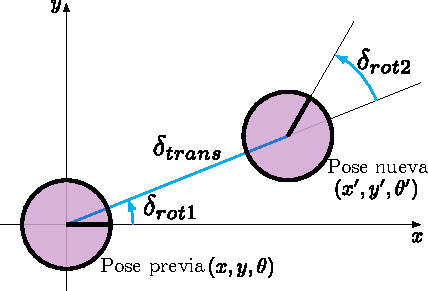
\includegraphics[width=0.5\textwidth]{./images/odometry_as_controls.pdf}
\caption{Motion model}
\label{fig:odometry-base-motion-model}
\end{figure}

\subsection{Code description}

The provided code is written in Python and depends on the \lstinline[style=bash]{NumPy} and \lstinline[style=bash]{Matplotlib} libraries.

\begin{itemize}
\item \lstinline[style=bash]{localization.py} --- main entry point for running experiments.
\item \lstinline[style=bash]{soccer_field.py} --- Implements the dynamic and observation model functions, as well as the noise models for both. Implement Jacobians here!
\item \lstinline[style=bash]{utils.py} --- Contains several plotting functions, as well as a useful function for normalizing an angle between $[-\pi, \pi]$.
\item \lstinline[style=bash]{policy.py} --- Contains a simple policy that you can safely ignore.
\item \lstinline[style=bash]{ekf.py} --- Implement the Extended Kalman Filter here!
\item \lstinline[style=bash]{pf.py} --- Implement the Particle Filter here!
\end{itemize}

\subsection{Command Interface}

To visualize the robot in the soccer field environment, run

\begin{lstlisting}[style=bash]
python localization.py --plot none
\end{lstlisting}

The {\color{blue}} line plots the robot's position (ground-truth), which is the result of noisy actions. The {\color{green}} line plots the robot's position assuming the actions are not noisy (desired trajectory, but not the actual one). After implementing a filter, the robot's position estimated by the filter will be plotted in {\color{red}}.

\begin{lstlisting}[style=bash]
python localization.py --plot ekf
python localization.py --plot pf
\end{lstlisting}

To see the available command-line flags, run

\begin{lstlisting}[style=bash]
python localization.py -h
\end{lstlisting}

\subsection{Data Format}

\begin{itemize}
\item state: $[x,y,\theta]$
\item control: $[\delta_{rot1},\delta_{trans},\delta_{rot2}]$
\item observation: $[\theta_{bearing}]$
\end{itemize}

\subsection{Notes}
\begin{itemize}
\item Call \lstinline[style=bash]{utils.minimized_angle} whenever an angle or angle difference might exceed $[-\pi, \pi]$.
\item Use the low-variance systematic sampler seen in class. It gives a smoother particle distribution and also requires a single random number per resampling step.
\item Disable visualization to speed up execution.
\end{itemize}

\ejercicio Implementing EKF

Implement the Extended Kalman Filter algorithm in \lstinline[style=bash]{ekf.py}. You will need to complete \lstinline[style=bash]{ExtendedKalmanFilter.update} and the $G$, $V$, and $H$ methods. The results of a successful EKF implementation should be comparable to the following results.

\begin{lstlisting}[style=bash]
python localization.py ekf --seed 0
...
Mean position error: 8.9983675360847
Mean Mahalanobis error: 4.416418248584298
ANEES: 1.472139416194766
\end{lstlisting}

	\begin{enumerate}
\item Plot the actual robot path and the path estimated by the filter with the default parameters (provided).
\item Plot the mean position error as the factors $\alpha$ and $\beta$ vary over $r = [1/64, 1/16, 1/4, 4, 16, 64]$\footnote{Since the factors multiply with variances, this is between 1/8 and 8 times the default noise values.} and analyze the results obtained.

Run 10 trials per value of $r$. An execution might look something like this:

\begin{lstlisting}[style=bash]
python localization.py ekf --data-factor 4 --filter-factor 4
\end{lstlisting}

\item Plot the mean position error and ANEES (\emph{average normalized estimation error squared}) as the filter factors $\alpha$, $\beta$ vary over $r$ (as above) while the data is generated with the default values. Analyze the results.
\end{enumerate}

\ejercicio Implementing PF

Implement the Particle Filter algorithm in \lstinline[style=bash]{pf.py}. You must complete \lstinline[style=bash]{ParticleFilter.update} and \lstinline[style=bash]{ParticleFilter.resample}.

\begin{lstlisting}[style=bash]
python localization.py pf --seed 0
...
Mean position error: 8.567264372950905
Mean Mahalanobis error: 14.742252771106532
ANEES: 4.914084257035511
\end{lstlisting}

\begin{enumerate}
\item Plot the actual robot path and the path estimated by the filter with the default parameters.
\item Plot the mean position error as the factors $\alpha$, $\beta$ vary over $r$ and discuss the results.
\item Plot the mean position error and ANEES as the filter factors $\alpha$, $\beta$ vary over $r$ while the data is generated with the default values.
\item Plot the mean position error and ANEES as the factors $\alpha$, $\beta$ vary over $r$ and the number of particles varies over $[20, 50, 500]$.
\end{enumerate}

	\printbibliography
	
\end{document}
